\section{Realisierung einer SOA}
\label{ch:realization}

% Aufteilung in Services

Es gibt viele unterschiedliche Wege eine SOA in der Praxis zu realisieren. Eine der verbreitetsten Möglichkeiten eine serviceorientierte Architektur zu realisieren ist mit Web-Services. Weitere Technologien zur Implementierung von SOA ist der Komponentendienst COM+ von Microsoft, Java 2 Platform Enterprise Edition (J2EE) oder die CORBA-Spezifikation. Im Folgenden werden jedoch nur Web-Services betrachtet, da dies der verbreitetste Weg ist eine SOA zu implementieren.


\begin{figure}[H]
    \centering
    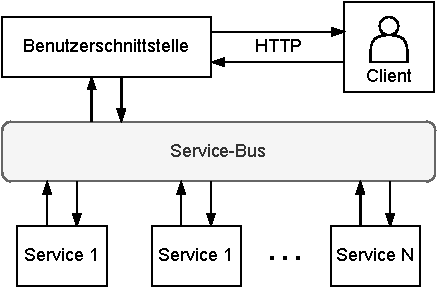
\includegraphics[width=.7\textwidth]{images/SOA-Service-Bus.drawio.pdf}
    \caption{SOA Aufbau}
    \label{fig:soa-aufbau}
\end{figure}

Wichtig zu sagen ist noch, dass es nicht nur einen richtigen Weg gibt, eine SOA zu implementieren. Es gibt meist viele verschiedene Wege, welche zum gewünschten Ziel führen können. In der Regel müssen mehrere Services implementiert werden, welche gemeinsam über einen Service-Bus miteinander kommunizieren können. Je nach expliziter Implementierung ist der Service-Bus dabei eine globale Instanz über die gesamte Applikation hinweg, oder eine Abstraktion für direkte Verbindungen zwischen verschiedenen Services. In Abbildung \ref{fig:soa-aufbau} wird ein beispielhafter Aufbau einer serviceorientierten Architektur dargestellt. Der Service-Bus ist dabei eine Abstraktion der Schnittstellen und an ihn angebunden sind verschiedene Service-Komponenten. Einer der Services ist dabei die Benutzerschnittstelle, mit der die Benutzer zum Beispiel über ein Frontend interagieren können.

\textbf{Service-Bus}

Mit der wichtigste Bestandteil eines Services ist seine Schnittstelle. Für die Realisierung der Schnittstelle kommen zwei verschiedene Designprinzipen infrage. Entweder ein nachrichtenorientiertes Design oder ein hypermedia-gesteuertes Design.\\
Bei dem nachrichtenorientierten Design kommunizieren die Services über einen Service-Bus. Über diesen können die einzelnen Komponenten Nachrichten austauschen. In der Regel wird dabei ein Message-Broker oder eine direkte Kommunikation der Services über TCP/IP verwendet. Für die Kommunikation zum Konsumenten wird in der Regel eine HTTP-API bereitgestellt.\\
Die zweite Möglichkeit ist die hypermedia-gesteuerte Implementierung. Im Gegensatz zur nachrichtenorientierten Implementierung werden bei der hypermedia-gesteuerten Implementierung nicht nur Daten, sondern auch Inhalte mit Beschreibungen möglicher Aktionen ausgetauscht. Dabei wird zum Beispiel direkt HTML Quelltext mit einer Form zurückgegeben. Dies ist vorteilhaft, wenn der Konsument über eine Webseite auf einen Service zugreifen will. \cite{NADAREISHVILI.2016}

Für die eigentliche Implementierung von dem Service-Bus gibt es viele Möglichkeiten. Ein Service-Bus kann beispielsweise als separate Software-Komponente implementiert werden. Der Service-Bus kann dabei von Grund auf implementiert werden oder es kann ein bestehender Message-Broker wie zum Beispiel RabbitMQ verwendet werden. Dabei kann der Service-Bus Nachrichten empfangen und über Routing an den richtigen Service weiterleiten. Der Vorteil daran ist, dass der Service-Bus dabei beliebig skaliert werden kann. Eine weitere Möglichkeit wäre eine in die Services integrierte Middleware, welche die benötigten Schnittstellen zur Kommunikation unter den Services zur Verfügung stellt. Dabei werden üblicherweise Web-Protokolle wie SOAP oder REST eingesetzt. \cite{Heutschi.2007}

% Service Provicer - Service Customer

% Service Bus
%   - Message Broker
%   - (REST) APIs
%   - IPC

% API Design:
%   - Nachrichtenorientiert
%   - Hypermedia-Driven
% https://docs.broadcom.com/doc/microservice-architecture-aligning-principles-practices-and-culture S. 67

% \subsection{Modellierung}

% Schnittstellenbasierte oder Komponentenbasierte Modellierung bietet sich an. Dafür bietet sich UML ab der Version 2.0 an, da dort wesentliche Verbesserungen in der Darstellung von Komponenten und Kontroll- und Ablaufkonzepte beinhaltet. 

% A Service Component is an encapsulated, autonomous software entitiy that realizes and provides the Service through its interface in a contract-based fashion without exposing its internal implementation

\textbf{Service-Komponente}

% Jede Service-Komponente erfüllt eine kleine Funktionalität der Applikation

Eine Service-Komponente ist eine Software-Entität, welche als eigenständige, unabhängige und in sich geschlossene Einheit mit einem klaren Zweck besteht. Die Komponente ist dabei eine unabhängige Einheit von einer Funktionalität mit standardisierten Schnittstellen zur Kommunikation mit anderen Komponenten in einer Anwendung. In der Regel hat die Service-Komponente eine eindeutige Funktion, welche unabhängig von anderen Service-Komponenten der Anwendung ist.

Die eigentliche Implementierung des Services kann in einer beliebigen Programmiersprache geschehen. Es können auch unterschiedliche Services in unterschiedlichen Programmiersprachen implementiert werden. Dabei kann individuell für die Funktionalität eines jeweiligen Services eine optimale Programmiersprache verwendet werden. Wichtig ist dabei lediglich, dass die Schnittstellen korrekt angesprochen werden.   

% Die Basiselemente einer Service-Komponente sind sein Kontext, Kontrakt und Realisierung. Die Rolle eines Services ist in seinem Kontrakt spezifiziert. Der Kontrakt wird durch die Realisierung der Service-Komponente realisiert, die durch eine Schnittstelle vor dem Kontext verborgen ist. Mehrere Service-Komponenten, welche im selben Kontext zusammenarbeiten, werden als Choreografie bezeichnet. In Abbildung \ref{fig:component-metamodell} ist das Service-Komponenten-Metamodell dargestellt. \cite{Stojanovic.op.2004}

% \begin{figure}[H]
%     \centering
%     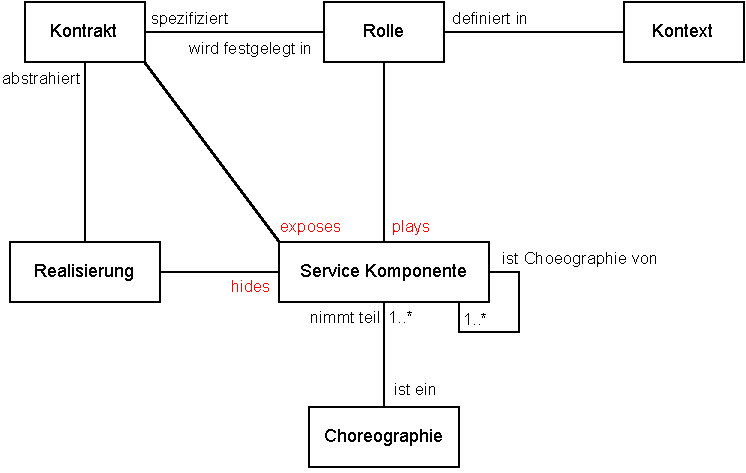
\includegraphics[width=1.\textwidth]{images/Service-Komponent-Metamodell.drawio.pdf}
%     \caption{Service-Komponenten-Metamodell}
%     \label{fig:component-metamodell}
% \end{figure}

\begin{figure}[H]
    \centering
    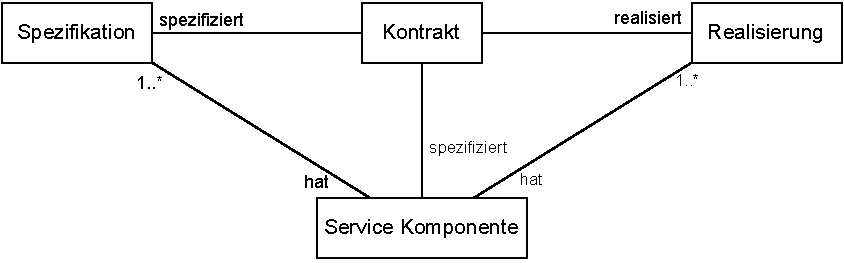
\includegraphics[width=1.\textwidth]{images/Spezifikation-Realisation-Service.drawio.pdf}
    \caption{Spezifikation und Realisation einer Service-Komponente \cite{Stojanovic.op.2004}}
    \label{fig:specification-realisation}
\end{figure}

Die Basiselemente für die Planung und Umsetzung einer Service-Komponente sind die Spezifikation, der Kontrakt und die Realisierung. Die Zusammenhänge der Basiselemente sind in Abbildung \ref{fig:specification-realisation} dargestellt. Im Kontrakt sind dabei die Regeln und Anforderungen der Service-Komponente spezifiziert. Also der Funktionsumfang, welcher der Service bereitstellen soll. Dieser Kontrakt wird in der Spezifikation weiter spezifiziert. In der Spezifikation wird die Art und die Verwendung der Schnittstellen definiert. Darunter zählen zum Beispiel die verwendeten Protokolle und Standards für die Kommunikation und die Information welche Funktionen von dem Service bereitgestellt werden. Wurde alles korrekt spezifiziert kann der Service-Kontrakt implementiert werden. Für die Benutzung des Services ist dessen Implementierung nicht von Bedeutung, solange der Kontrakt des Services voll erfüllt wurde. \cite{Stojanovic.op.2004}

\subsection{Konzepte und Technologien}
\label{sec:conceptsAndTechnologies}

In der serviceorientierten Architektur gibt es keine Vorschriften wie genau etwas zu implementieren ist und welche Technologie dabei verwendet werden soll. Jedoch gibt es einige Technologien und Konzepte, welche sich in dem Bereich der SOA etabliert haben. Die Wahl der explizit zu verwendeten Technologien ist dabei von den Anforderungen der Anwendung abhängig. Bei der Planung und dem Design sollten die Technologien jedoch genau spezifiziert werden, welche anschließend zur Implementierung verwendet werden.

Die verbreitetste Technologie zur Umsetzung von SOA sind Web-Services. Web-Services kommunizieren über standardisierte Schnittstellen in einem Netzwerk miteinander. Dabei funktioniert die Kommunikation über Netzwerkprotokolle wie zum Beispiel SOAP oder REST. \cite{Heutschi.2007}

\begin{figure}[H]
    \centering
    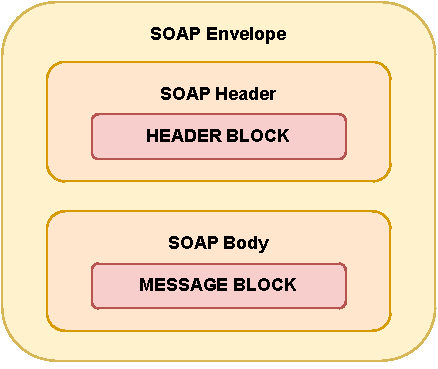
\includegraphics[width=.5\textwidth]{images/SOAP.drawio.pdf}
    \caption{SOAP Aufbau \cite{AlexanderS.Gillis.02.12.2022}}
    \label{fig:soap}
\end{figure}


Das Simple Object Access Protocol (SOAP) benutzt in der Regel das HTTP-Protokoll zur Datenübertragung. Dabei werden die Daten in Form von XML gesendet. SOAP ist unabhängig von der verwendeten Programmiersprache und wird meist in verteilten Systemen und somit auch in SOA verwendet. Der Aufbau einer SOAP-Komponente ist in Abbildung \ref{fig:soap} dargestellt. Außen befindet sich der SOAP Envelope, welcher alle Daten enthält und das XML-Dokument als SOAP-Nachricht identifiziert. In dem SOAP Envelope befindet sich ein Header und ein Body. Der Header beinhaltet dabei zusätzliche Informationen über die Nachricht. Dies sind zum Beispiel zusätzliche Daten zur Authentifizierung. Im Body steht der eigentliche Inhalt der Nachricht. SOAP kann sowohl für Anfragen an einen Service, als auch für dessen Antwort verwendet werden. \cite{AlexanderS.Gillis.02.12.2022}

Der Aufbau in Abbildung \ref{fig:soap} wird wie folgt im XML-Format geschrieben: 

\begin{lstlisting}
<?xml version="1.0"?>
<soap:Envelope xmlns:soap="http://www.w3.org/2003/05/soap-envelope/">
    <soap:Header>
        HEADER BLOCK
    </soap:Header>
    <soap:Body>
        MESSAGE BLOCK
    </soap:Body>
</soap:Envelope>
\end{lstlisting}

Um einen Service und vor allem dessen Schnittstellen zu beschreiben kann die Web Services Description Language (WSDL) verwendet werden.\\
WSDL ist ein Standardformat um einen Web-Service zu beschreiben. Die Beschreibung des Services wird in dem XML-Format in der WSDL-Datei definiert. Neben einer Beschreibung der Funktionalität des Services sind auch alle Informationen, um mit einem dem Web-Service zu kommunizieren, darin enthalten. \cite{Heutschi.2007}

Häufig wird WSDL in Verbindung mit SOAP verwendet. Dabei kann der Client, welcher den Service anfragt, die WSDL Datei einlesen, um somit die verfügbaren Funktionen des Services abzurufen. Nun kann er die in WSDL definierten verfügbaren Funktionen über das SOAP-Protokoll verwenden. \cite{Heutschi.2007}

Für die Umgebung, in der die Services ausgeführt werden, bietet sich eine skalierbare Cloud-Infrastruktur an, bei der eine schnelle Bereitstellung an Rechenkapazitäten und ein automatisches Deployment der Services realisiert werden kann. 

% WSDL:
% - Standardformat um einene Web-Service zu beschreiben
% - XML-Datei
% - beinhaltet alle Informationen um mit einem Web-Service zu kommunizieren  (Interface)
% - Beschreibt die Funktionalität eines Web-Services

% Web Services: WSDL, SOAP
% Messaging: RabbitMQ
% REST
% OPC-UA

% - Programmiersprache, welche web API freundlich ist
% - Programmiersprache, welche den Kompetenzen des Entwicklerteams entspricht
